\documentclass[english, twocolumn, 10pt, aps, superscriptaddress, floatfix, prb, citeautoscript]{revtex4-1}
\pdfoutput=1
\usepackage[utf8]{inputenc}
\usepackage[T1]{fontenc}
\usepackage{verbatim}
\usepackage{units}
\usepackage{mathtools}
\usepackage{amsmath}
\usepackage{amssymb}
\usepackage{graphicx}
\usepackage{wasysym}
\usepackage{layouts}
\usepackage{siunitx}
\usepackage{bm}
\usepackage{xcolor}
\usepackage[colorlinks, citecolor={blue!50!black}, urlcolor={blue!50!black}, linkcolor={red!50!black}]{hyperref}
\usepackage{bookmark}
\usepackage{tabularx}
\usepackage{microtype}
\usepackage{babel}
\hypersetup{pdfauthor={Quantum Tinkerer},pdftitle={Increasing the topological gap by an order of magnitude through the geomerty for Majorana SNS junctions.}}

\setcounter{secnumdepth}{4}
\setcounter{tocdepth}{4}

\DeclareMathOperator{\e}{e}
\DeclareMathOperator{\de}{d\!}
\DeclareMathOperator{\Tr}{Tr}
\DeclareMathOperator{\diag}{diag}
\DeclareMathOperator{\Res}{Res}
\DeclareMathOperator{\sgn}{sgn}
\DeclareMathOperator{\Pf}{Pf}
\DeclareMathOperator{\Det}{Det}
\DeclareMathOperator{\rank}{rank}
\DeclareMathOperator{\im}{Im}
\DeclareMathOperator{\re}{Re}
\newcommand{\kx}{k_x}
\newcommand{\ky}{k_y}
\newcommand{\meff}{m_\text{eff}}

\renewcommand{\comment}[2]{#2}
% Uncomment the following line for paragraph descriptions to appear in the file.
\renewcommand{\comment}{\paragraph}

\DeclarePairedDelimiter\abs{\lvert}{\rvert}
\DeclarePairedDelimiter\norm{\lVert}{\rVert}

\makeatletter
\let\oldabs\abs
\def\abs{\@ifstar{\oldabs}{\oldabs*}}
\let\oldnorm\norm
\def\norm{\@ifstar{\oldnorm}{\oldnorm*}}
\makeatother

\newcommand{\ev}[1]{\langle#1\rangle}
\newcommand{\bra}[1]{\langle#1|}
\newcommand{\ket}[1]{|#1\rangle}
\newcommand{\bracket}[2]{\langle#1|#2\rangle}

\newcolumntype{L}[1]{>{\raggedright\arraybackslash}p{#1}}
\newcolumntype{C}[1]{>{\centering\arraybackslash}p{#1}}
\newcolumntype{R}[1]{>{\raggedleft\arraybackslash}p{#1}}


\begin{document}


\title{Increasing the topological gap by an order of magnitude through the geometry for Majorana SNS junctions.}

\author{Quantum Tinkerer}
\affiliation{Kavli Institute of Nanoscience, Delft University of Technology, P.O. Box 4056, 2600 GA Delft, The Netherlands}
\email[Electronic address: ]{quantumtinkerer@tudelft.nl}

\date{\today}

\begin{abstract}
We are solving a problem of soft gap in high density SNS Majorana junctions \cite{pientka2017topological}.
We do this by introducing a zigzag geometry.
This works because the maximum trajectory length is cut-off due to the geometry and therefore the minimal energy gap is given by a simple formula, which we also verify using numerics.
In addition to having a large minimum energy gap, the absence of long length trajectories means that the localization length is very short as well.
\end{abstract}

\maketitle

%%██████████████████████████████████████████████████████████████████████████
%%██ Introduction
%%██████████████████████████████████████████████████████████████████████████
\section{Introduction}
Majorana bound states (MBSs) are a promising candidate to form the basis of a stable platform for topological quantum computing.

\comment{Majoranas are mostly made in hybrid NS structures.}
The current experimental effort is focused on creating pairs of MBSs in hybrid normal-superconductor (NS) structures, where a lengthy strip (or wire) of semiconductor is interfaced with a \cite{lutchyn_majorana_2010,oreg_helical_2010} superconductor.
Within the right parameter regime ($E_z^2>\mu^2+\Delta^2$ for a simple wire), the semiconductor becomes topological and MBSs appear at the ends of the segment.
Recently, a system with a slight modification has been proposed\cite{pientka2017topological}, where instead of having one superconductor, there are two superconductors, creating a superconductors-normal-superconductor (SNS) junction.
This adds an extra knob to adjust, the superconducting phase difference $\phi$, and this should make it easier to tune the system into the topological phase.
In practice, multiple problems arise making even the observation, let alone the manipulation of Majoranas difficult.

\comment{Currently proposed workarounds are low density or disorder, but both have drawbacks.}


\comment{The gap is small because of long trajectories.}
One of the biggest challenges in constructing stable Majoranas is the appearance of a soft gap; where the gap in the density of states is greatly reduced for states with momentum directed along the length of the strip.
From a semiclassical perspective, these momenta correspond to long paths through the semiconductor without interruption by the superconductor.
Additionally, these long trajectories have long flight times $\tau_f$ and equivalenly small Thouless energies $E_{\textrm{Th}}=\hbar / \tau_f$, resulting in a small gap. 

\comment{We show that zigzag geometry solves this problem by eliminating the long trajectories.}
In this paper we show that introducing a zigzag or snake like geometry for the semiconductor eliminates these long trajectories and prevents the appearance of a soft gap.


%%██████████████████████████████████████████████████████████████████████████
%%██ Physical picture
%%██████████████████████████████████████████████████████████████████████████
\section{Physical picture}

\comment{We consider a two-dimensional system with zigzag.}
We consider a system (Fig.~\ref{fig:setup}) consisting of a two dimensional strip of semiconductor, with superconductors on both sides.
We modulate the shape of the normal region, which can be either zigzag as depicted, or a more smooth sinusoidal like shape.
Similar to the straight system \cite{pientka2017topological}, a magnetic field $B_x$ pointed along the $x$ direction is applied.
We model the system with a BdG Hamiltonian Eq.~\eqref{eq:hamiltonian}; the normal part has Rashba spin-orbit coupling and a Zeeman field, and apart from the kinetic term, the superconductors only have a superconducting term with a superconducting phase.
For the zigzag geometry, we take a sawtooth like pattern where $z_x$ is periodicity, $z_y$ the amplitude and $W$ the width of the junction.

\comment{The symmetry class of the system is D.}
We know from \onlinecite{pientka2017topological} that the non-zigzag system is in class BDI.
Using the software package Qsymm\cite{varjas2018qsymm}, we evaluate the symmetry class of the system to be D.

\begin{small}
\begin{align}
    H = \left(\frac{\hbar^2\left(\kx^2 + \ky^2\right)}{2\meff} - \mu\right)\tau_z+
        E_\text{z} \sigma_x+
        \alpha \left( \ky \sigma_x - \kx \sigma_y \right) \tau_z +
        \Delta \tau_y
\end{align}
\label{eq:hamiltonian}
\end{small}

\begin{figure}[!htb]
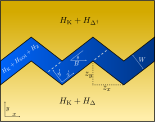
\includegraphics[width=0.95\columnwidth]{figures/zigzag.pdf}
\caption{Setups. Figure of a straight and zigzag system, including trajectories.
\label{fig:setup}}
\end{figure}

%%██████████████████████████████████████████████████████████████████████████
%%██ Calculating the bandstuctures
%%██████████████████████████████████████████████████████████████████████████
\section{Calculating the bandstuctures.}

\comment{We discretize the model described in section II and simulate it with Kwant.}
We implement a tightbinding version of the model described in section II (a two dimensional SNS junction with a Rashba BdG Hamiltonian) using Kwant.

\comment{We calculate the bandstructure for varying amount of zigzag.}
In figure \ref{fig:bandstuctures}, the bandstructure for zigzag systems with varying amplitude is displayed.
As the zigzag introduces super cell, we see a folded bandstructure.
For comparisons sake, we take the same cell size for the ribbon structure so the bandstructure is folded in the same way.

\comment{The bandstructures show that modulation of the geometry increases the gap by an order of magnitude, as well as reduce the group velocity.}
The introduction of a zigzag has a striking effect: the bands flatten out, and more importantly, the gap size is increased more than an order of magnitude.
This effect is due to the fact that the modes where the gap is smallest, when the momentum is almost completely focused along the strip ($k_x=k_F$), are cut off by the zigzag geometry.
Also apparent is the reduction of group velocity; the slope of the bands is greatly reduced.
This has an effect on the Majorana coherence length, as described later on in the manuscript.

\comment{The introduction of an SN interface at many angles also increases performance.}
Additionally in the presence of normal reflection, due to the availability of NS interfaces at a wide range of slopes, the reflected part will eventually ``find'' a surface with which it is perpendicular to. The transparency of the SN interface is thus improved for transversal modes.


%%██████████████████████████████████████████████████████████████████████████
%%██ Calculating the topological phase diagram
%%██████████████████████████████████████████████████████████████████████████
\section{Calculating the topological phase diagram.}

\comment{We calculate the topological phase diagram using the gap size.}
We calculate the gap from the bandstructure (minimum energy in the spectrum) using the same method described in comment III.
Noting the gap closings and the fact we know the topology for the non-zigzag system, we can infer the topology of the system with zigzag modulation.

\comment{The phase diagram does not change much, except we see a cleaner spectrum as a result of the D class symmetry. }
Similar to what is described in Pientka et. al [\cite{pientka2017topological}], we see that the ribbon topology has a diamond like structure as a function of phase and Zeeman field.
We also see some additional gap closings which are due to the BDI symmetry class, creating quite an unstable region.
As expected, for the zigzag system, the magnitude of the gap is significantly improved, whilst maintaining the diamond like shape.
As the zigzag shape destroys the additional symmetry, moving it to class D, we see a more clean topological region.

\begin{figure}[!htb]
\includegraphics[width=0.95\columnwidth]{figures/bandstructures}
\caption{Figure of the bandstuctures.
Where the lines are (blue) $\phi=0$, $B=0$ and (red) $\phi=\pi$, $B \ne 0$.
and the subplots (a) $z_y=0$, (b) $z_y=\frac{W}{4}$, and (c) $z_y=\frac{W}{2}$, where $W$ is the junction width.
We observe that once there are no more straight trajectories inside the junction (when $z_y=\frac{W}{2}$) the spectrum becomes most insensitive to the momentum $k_x$.
\label{fig:bandstuctures}}
\end{figure}

\begin{figure}[!htb]
\includegraphics[width=0.95\columnwidth]{figures/phasediagrams}
\caption{Phase diagrams of a straight system (a, b) and zigzag system (c, d), where (a, c) are $E(\mu, B)$ and (b, d) are $E(\phi, B)$.
We use a generalized eigenvalue problem to find all phase boundaries at once and find the minimal energy gap by finding the minimum in the spectrum: $\min{E(k)}$.
\label{fig:phasediagrams}}
\end{figure}

%%██████████████████████████████████████████████████████████████████████████
%%██ Analytical estimate
%%██████████████████████████████████████████████████████████████████████████
\section{Analytical estimate of the band gap}

\comment{To compute the effect of cutoff consider a single segment of the zigzag and obtain the spectrum analytically (this allows to use translation invariance).}
We establish that the cutoff of long trajectories is the driving mechanism behind the order of magnitude gap improvement using an analytical approach.
We derive the Andreev spectrum for a single (diagonal) segment of the zigzag, and define the gap of the system as the minimum of the spectrum occurring before the cutoff corresponding to the particular geometry.
The system under consideration is thus a ribbon SNS junction with tilted magnetic field.

\comment{The definition of the cutoff... }

\comment{We use a short junction approximation and neglect transverse SO.}
We derive the spectrum by calculating the scattering matrix for the normal region and applying the Andreev bound state condition for the short junction limit\cite{beenakker1991universal, sticlet_robustness_2017}. 
For deriviation of the scattering matrix, we neglect SOI in the transverse direction, which is valid for $W<l_\text{so}$.
The result is specified in Eqs. \ref{eq:smatrix} to \ref{eq:momenta_short_junction}.

\begin{align}
\label{eq:smatrix}
    S &= \left(
    \begin{array}{rr}
    r_{ll}&t_{rl}\\
    t_{lr}&r_{rr}\\
    \end{array}
    \right) =
    \left(
    \begin{array}{rr}
    \beta_+ & e^{-i q W} \beta_-\\
    e^{-i q W} \beta_- & e^{-2 i q W} \beta_+\\
    \end{array}
    \right)
    \\
    \beta_\pm &= \left(
    \begin{array}{rr}
    e^{i \nu_{\arg}}\left(\omega^\pm_1 - \omega^\pm_2\right) & (\omega^\pm _1 + \omega^\pm _2)\\
    -(\omega^\pm _1 + \omega^\pm _2) & e^{-i \nu _{\arg }} \left(\omega^\pm _2 - \omega^\pm _1\right)\\
    \end{array}
    \right)\\
    \omega^\pm_j &= \frac{1}{4} \left(\gamma _{j} \pm \delta _{j}\right)
\end{align}

\begin{align}
    \gamma_j &= \frac{q+i k_{j} \tan \left(\frac{W k_{j}}{2}\right)}{q-i k_{j} \tan \left(\frac{W k_{j}}{2}\right)} \\
    \delta_j &= \frac{q-i k_{j} \cot \left(\frac{W k_{j}}{2}\right)}{q+i k_{j} \cot \left(\frac{W k_{j}}{2}\right)}\\
    e^{i \nu_{\arg}} &= \frac{E_\text{z} e^{i \theta }-i \alpha  k_x}{\sqrt{E_\text{z}^2+\alpha  k_x \left(\alpha  k_x-2 E_\text{z} \sin (\theta )\right)}}
\end{align}

\begin{footnotesize}
\begin{align}
    q &= \left[ \frac{2 m_\ast}{\hbar ^2}\mu_s - k_x^2 \right]^\frac{1}{2}\\
    k_1 &= \left[ \frac{2 m_\ast}{\hbar^2} \left(\mu_n-\sqrt{E_z^2-2 \alpha  E_z \sin (\theta ) k_x+\alpha ^2 k_x^2}\right) - k_x^2 \right]^\frac{1}{2}\\
    k_2 &= \left[ \frac{2 m_\ast}{\hbar^2} \left(\mu_n+\sqrt{E_z^2-2 \alpha  E_z \sin (\theta ) k_x+\alpha ^2 k_x^2}\right) - k_x^2 \right]^\frac{1}{2}
\label{eq:momenta_short_junction}
\end{align}
\end{footnotesize}


In order to get the spectrum from the S-matrix [Eq.~\eqref{eq:smatrix}] we use the main result from Ref.~\onlinecite{beenakker1991universal} and start with a determinantal equation for the bound state energies in a SNS-junction:

\begin{equation}
\det\left[1+\alpha^{2}\left(E\right)r^{*}S_{e}\left(E,\bm{k}\right)rS_{e}^{*}\left(-E,-\bm{k}\right)\right]=0
\end{equation}

We rewrite this as a characteristic polynomial problem $\det\left[A-\lambda I\right]=0$, as

\begin{equation}
\det\left[r^{*}S_{e}\left(E,\bm{k}\right)rS_{e}^{*}\left(-E,-\bm{k}\right)-\frac{-1}{\alpha^{2}\left(E\right)}I\right]=0
\end{equation}

with
\begin{equation}
\lambda=-\frac{1}{\alpha^{2}\left(E\right)},\;A=r^{*}S_{e}\left(E,\bm{k}\right)rS_{e}^{*}\left(-E,-\bm{k}\right).
\end{equation}

Where $\lambda_i$ are the eigenvalues of $A$.
Inverting $\alpha\left(E\right)\equiv\exp\left(-i\arccos\left(E/\Delta\right)\right)$ yields $\frac{E}{\Delta}=\frac{\alpha^{2}+1}{2\alpha}=\frac{1}{2}\left(\alpha+\alpha^{-1}\right)=\textrm{Re}(\alpha)$, where the last equality holds because $\alpha$ is unitary.
Then, since $\alpha$ is only defined in the positive imaginary plane, the energies are $\frac{E_{i}}{\Delta}=\textrm{Re}\left(\sqrt{-1/\lambda_{i}}\right)$ where we take the root which has a positive imaginary part.
Using this result and Eq.~\eqref{eq:smatrix}, we numerically find the Andreev spectrum.

\comment{The lowest energy at $|k| < k_\textrm{cutoff}$ sets the band gap.}
We cut off the spectrum at the momentum corresponding to the proposed cutoff in the zigzag, and compare it to the numerically obtained gap for a true zigzag system.

%%██████████████████████████████████████████████████████████████████████████
%%██ Localization lengths and shape effect
%%██████████████████████████████████████████████████████████████████████████
\section{Localization lengths and shape effects}

\comment{In a zigzag geometry Majoranas are localized within one segment of zigzag.}

\comment{We find the Majorana lengths by calculating the slowest decaying mode.}
Using the tight-binding package Kwant~\cite{groth_kwant:_2014}, we model a finite system to compute the Majorana wave function density for different geometries; ribbon, zigzag, parallel curve and vertically offset sinusoids.
In figure \ref{fig:wavefunctions} the wavefunctions are displayed, superimposed upon their respective geometry.
For the ribbon system, we see that the Majorana coherence length is relatively large, not showing the decolalized nature sought after.
All of the zigzag type geometries however show greatly reduced coherence length.
This can be explained by two effects: the increase in topological gap, but also the before mentioned reduction of the group velocity.

\comment{We also confirm that the specific shape does not matter.}
Also note the similarity between the various shapes, sharp corners or more smoothlike, the effect is the same.

\begin{figure}[!htb]
\includegraphics[width=0.95\columnwidth]{figures/wavefunctions}
\caption{Wavefunctions for different sizes and geometries.
With (a) a straight system, (b) a zigzag system, (c) a system where the normal region is defined by lines parallel to a sinosoid, and (d) a system with vertically offset sinosoids.
Inside the figure we indicate the Majorana length (or coherence length) $\xi$ and the topological energy gap $E_\textrm{gap}.$
We observe that $\xi$ for (a) is orders of magnitude longer and $E_\textrm{gap}$ orders of magnitude smaller than for (b, c, d), meaning that the details of the geometry do not matter.
\label{fig:wavefunctions}}
\end{figure}

%%██████████████████████████████████████████████████████████████████████████
%%██ Discussion and Conclusions
%%██████████████████████████████████████████████████████████████████████████
\section{Discussion and Conclusions}

\comment{The zigzag geometry is a useful tool in hardening the gap and decreasing majorana length, now experimental verification necessary}
Modulating the geometry of the normal ribbon solves the problems of gap softening and majorana length in an effective and controllable manner.
Additionally, the breaking of BDI symmetry into D symmetry results in a cleaner phase diagram.

\comment{Current fabrication techniques seem compatible with the proposed geometry, and experimental verification should point out whether it holds up to its promise.}
Current fabrication techniques seem compatible with the proposed geometry, and experimental efforts are already on their way.
Apart from optimizing the geometry for gap and Majorana length, the same freedom of geometry we use can additionally be applied to ease experimental implementation.
Slight modifications to the geometry, for example to ease measurement, should not have large implications on the physics.

\comment{It would be interesting to study what geometry creates an optimal environment for Majorana modes to exist.}
We have studied sawtooth, snake like and offset sinosoid modulation of the semicondctor region, but perhaps a more exotic shape will be optimal.
A systematic study of the effect of specific geometrical features would be interesting to study.

\comment{Extensions: we omit several physical effects, disorder, electrostatics, etc.}
We omit several physical effects, such as: disorder, electrostatics, the orbital effect, etc..
Experimental verification, along with further study of the proposed system is required to see whether their omittance obscure the improvements in the model studied in this manuscript.

\comment{Outlook: how to cope with the complications.}

\comment{Acknowledgments}

We are grateful to "people" for useful discussions.
This work was supported by the Netherlands Organization for Scientific Research (NWO/OCW), as part of the Frontiers of Nanoscience program, the Foundation for Fundamental Research on Matter (FOM), and an ERC Starting Grant STATOPINS 638760.

\bibliographystyle{apsrev4-1}
\bibliography{snakemajoranas}
\end{document}
